\subsection{Sensors}

\subsubsection{Landmine Detection Techniques}

Landmine detection technologies have evolved to encompass a wide range of sensing principles, each targeting specific physical, chemical, or biological characteristics of surface-laid and buried mines. Broadly, these methods can be categorized into five general classes: \textit{\textbf{electromagnetic induction-based} techniques}, \textit{\textbf{radiowave and microwave-based} systems}, \textit{\textbf{spectral and thermal imaging} approaches}, \textit{\textbf{mechanical and vibro-acoustic} methods}, and \textit{\textbf{chemical and biological} sensing methods}. Within each class, a variety of specialized detection technologies have been developed, including traditional metal detectors, ground-penetrating radar, infrared and hyperspectral imaging, seismic/acoustic sensors, vapor detection, and biosensors. Each of these approaches offers distinct advantages and faces specific limitations, especially when adapted to drone-based platforms for remote and efficient minefield scanning. In the following subsections, each class is explored in detail, with emphasis on the operating principles, detection capabilities, challenges, and documented UAV-based applications.

\paragraph{Electromagnetic Induction-Based Techniques}

Electromagnetic induction (EMI) methods operate by exploiting the interaction between electromagnetic fields and conductive or magnetic materials in the ground. These systems are typically composed of a transmitter coil that emits a time-varying electromagnetic field into the soil. When this field encounters a conductive object—such as a landmine with metallic components—it induces eddy currents within the object, which in turn generate a secondary magnetic field. This field is detected by a receiver coil, and the resulting signal is processed to infer the presence of the object. These principles form the basis of conventional \textbf{metal detectors}~\cite{gichd2006guidebook}.

In contrast, \textbf{magnetic sensors} or magnetometers do not actively induce eddy currents but instead measure disturbances in the Earth's ambient magnetic field caused by nearby ferromagnetic objects. While metal detectors rely on electromagnetic induction to detect a wide range of conductive materials, magnetometers are primarily sensitive to ferrous (iron-containing) materials and are particularly effective in detecting anomalies in the magnetic environment\footnote{\label{magnetometerfootnote}\url{https://www.sphengineering.com/integrated-systems/technologies/magnetometer}}.

Several specialized EMI sensors have been developed, including induction coil imaging systems that generate spatial maps of subsurface metallic objects, conductivity meters that monitor variations in soil conductivity through eddy current decay, and a range of magnetometers such as fluxgate, proton precession, optically pumped atomic, and meandering winding designs. Each sensor type offers specific trade-offs in sensitivity, resolution, and robustness, and may be selected based on the expected mine characteristics and deployment constraints~\cite{Gooneratne2004ARO, Bruschini1997ASO}.


\textbf{Drone-Based Applications:} EMI sensors have been successfully integrated into UAV platforms in numerous studies~\cite{yoo2020drone,yoo2021application,rs16162916,Yoo2024UnmannedAV}. These include implementations of both lightweight metal detectors and magnetic sensors for aerial surveying of minefields. Figure~\ref{fig:metal_detector_drone} shows an example of a UAV equipped with a metal detector for low-altitude scanning, while Figure~\ref{fig:magnetometer_drone} illustrates a UAV-mounted magnetometer designed for aerial magnetic anomaly detection. 

\begin{figure}[h!]
    \centering
    \begin{subfigure}[b]{0.48\linewidth}
        \centering
        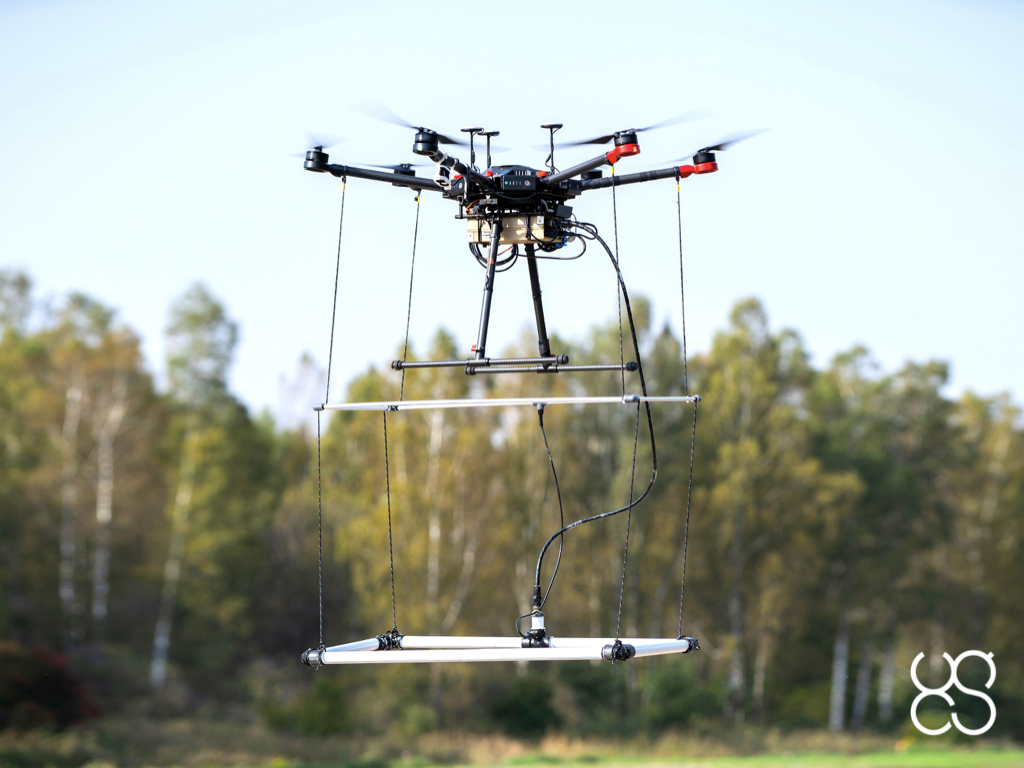
\includegraphics[width=\linewidth]{figs/Huirui/metal_detector_drone.png}
        \caption{UAV-mounted metal detector system\protect\footnotemark.}
        \label{fig:metal_detector_drone}
    \end{subfigure}
    \hfill
    \begin{subfigure}[b]{0.48\linewidth}
        \centering
        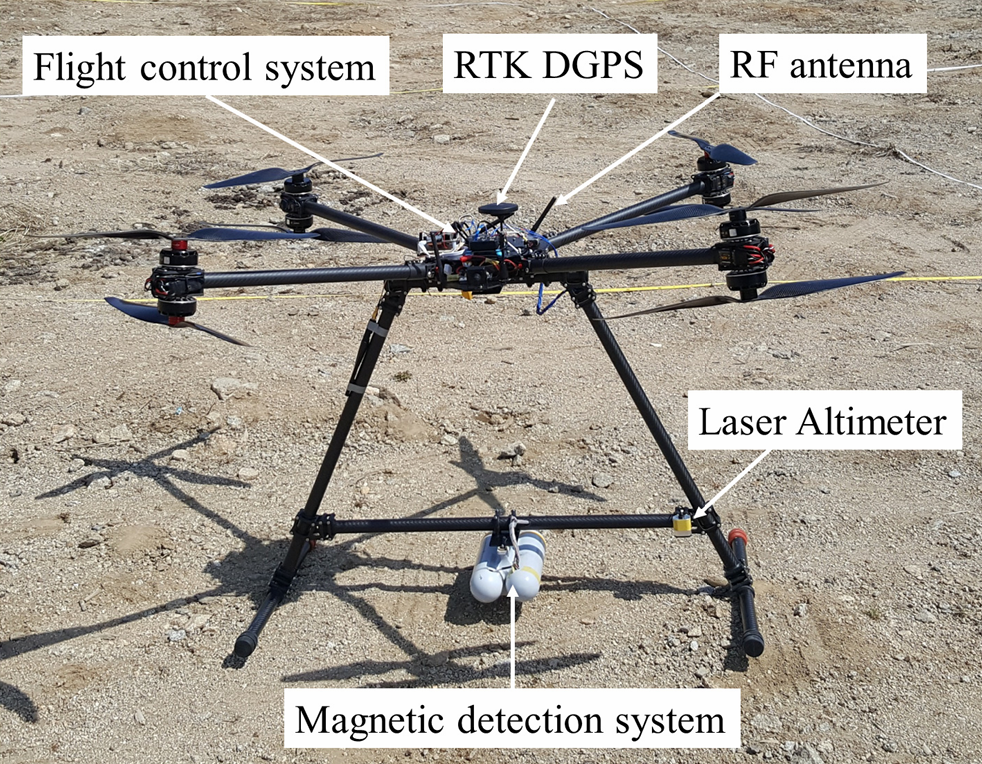
\includegraphics[width=\linewidth]{figs/Huirui/magnetometer_drone.png}
        \caption{Drone-based magnetometer platform~\cite{yoo2020drone}.}
        \label{fig:magnetometer_drone}
    \end{subfigure}
    \caption{Examples of UAV platforms integrating electromagnetic sensors for landmine detection.}
    \label{fig:emi_uav_examples}
\end{figure}

\footnotetext{\url{https://www.sphengineering.com/news/sph-engineering-introduces-the-drone-integrated-metal-detection-system}}

\paragraph{Radiowave and Microwave-Based Systems}

Ground Penetrating Radar (GPR) is a non-invasive geophysical technique that uses electromagnetic waves in the microwave frequency range (typically from several hundred MHz to a few GHz) to detect subsurface anomalies~\cite{gichd2006guidebook}. Unlike EMI-based systems, which respond to conductive or magnetic properties, GPR is sensitive to variations in the dielectric properties of materials~\cite{Gooneratne2004ARO}. It operates by transmitting short-duration radio pulses into the ground via a wideband antenna. When these pulses encounter boundaries between materials with different dielectric constants—such as between soil and a buried landmine—they are partially reflected. The reflected signals are then captured by a receiving antenna, and the time delay and intensity are analyzed to estimate the depth, shape, and dielectric contrast of subsurface targets~\cite{alqudsi2021review, paik2002image}.

As the antenna is moved across the ground, successive measurements are combined to construct two-dimensional slices (radargrams) or even three-dimensional volumetric representations of the subsurface~\cite{Bruschini1997ASO}. The effectiveness of GPR depends heavily on the contrast between the dielectric properties of the object and the surrounding soil. High-frequency systems offer better resolution and are more suited for detecting small anti-personnel mines, while lower-frequency systems provide deeper penetration but at the cost of detail~\cite{gichd2006guidebook}.


\textbf{Drone-Based Applications:} GPR has been widely explored for drone integration due to its capability to detect plastic-cased mines and to provide volumetric subsurface data. UAV-mounted GPR systems typically use lightweight ultra-wideband (UWB) antennas and operate at low altitude to maintain signal fidelity. Applications include detecting anti-tank and anti-personnel mines in varied terrain types, including sand, loam, and clay ~\cite{cerquera2017uav,vsipovs2020lightweight,colorado2017integrated,garcia2020airborne,garcia2019autonomous,burr2018design,fernandez2021development,lee2023modeling,sipos2017drone,garcia2022safedrone,schartel2018uav,chen2023ground}. Figure~\ref{fig:gpr_uav_examples} shows two UAV-based implementations of GPR for landmine detection.

\begin{figure}[h!]
    \centering
    \begin{subfigure}[b]{0.48\linewidth}
        \centering
        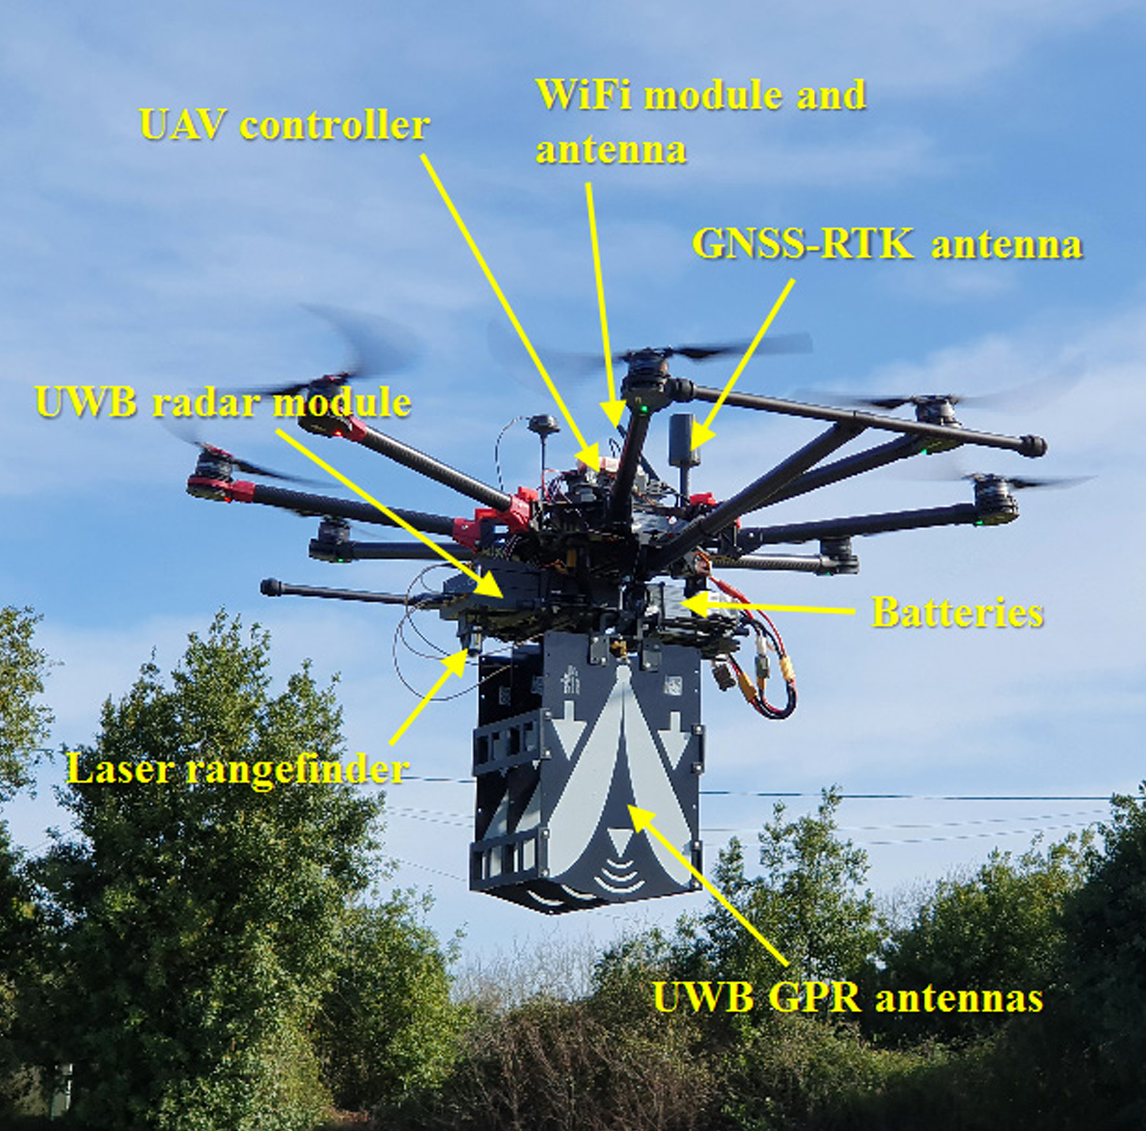
\includegraphics[width=\linewidth]{figs/Huirui/gpr_drone1.png}
        \label{fig:gpr_drone1}
    \end{subfigure}
    \hfill
    \begin{subfigure}[b]{0.48\linewidth}
        \centering
        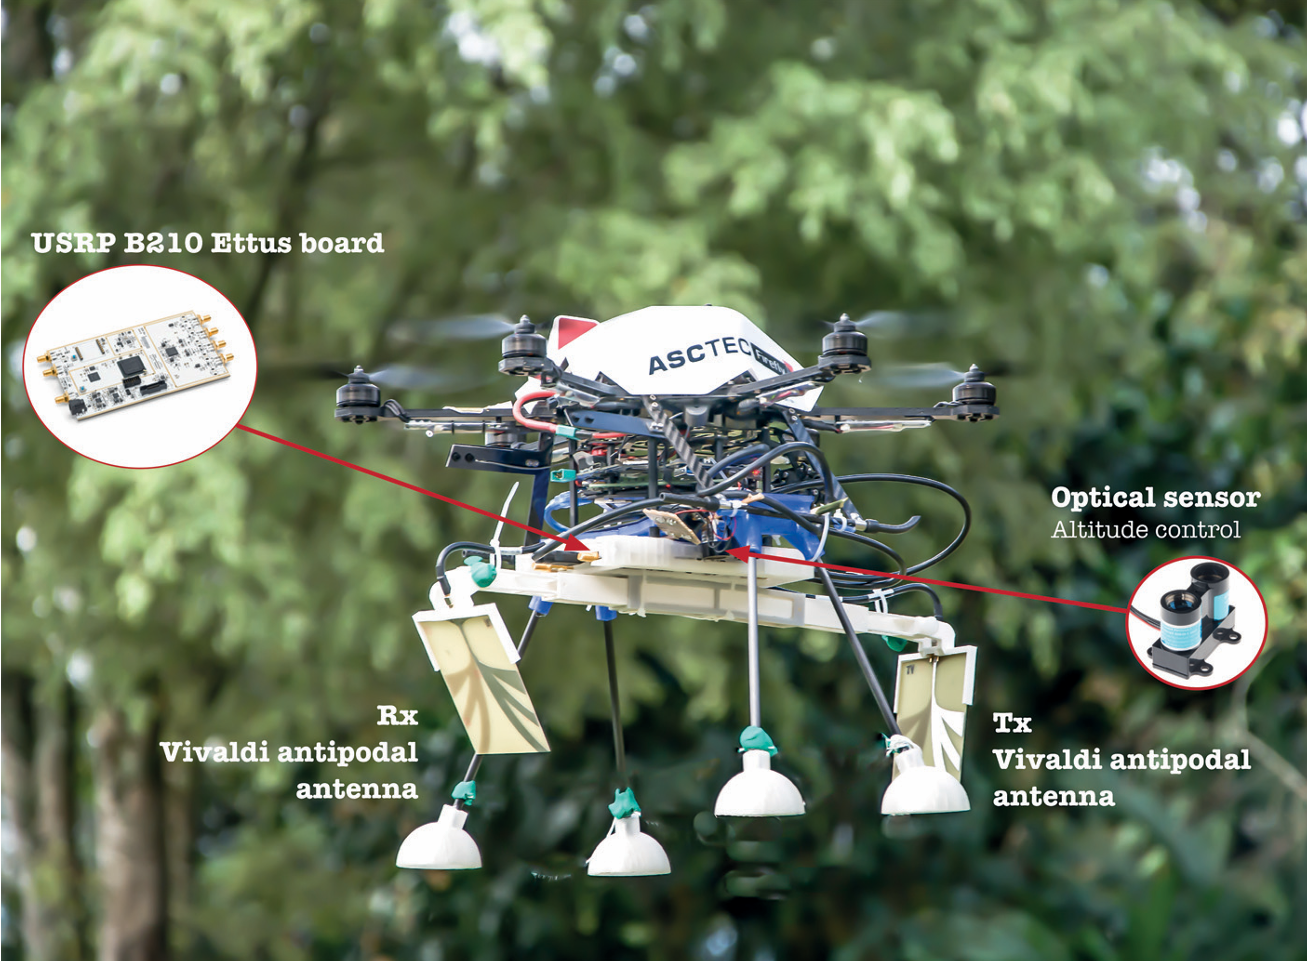
\includegraphics[width=\linewidth]{figs/Huirui/gpr_drone2.png}
        \label{fig:gpr_drone2}
    \end{subfigure}
    \caption{Examples of UAV platforms integrating GPR systems for landmine detection.~\cite{garcia2022safedrone,cerquera2017uav}}
    \label{fig:gpr_uav_examples}
\end{figure}

\paragraph{Spectral and Thermal Imaging Approaches}

Spectral and thermal imaging techniques detect anomalies in the electromagnetic radiation reflected or emitted from the Earth's surface. These methods aim to identify visual or thermal patterns associated with landmines or disturbed soil above them. The three primary sensor modalities in this class include visible-spectrum (optical) imaging, thermal infrared (IR) imaging, and hyperspectral or multispectral imaging.

\textbf{Optical cameras} operate in the visible light range and capture color or grayscale images of the terrain. They are primarily used to identify surface-laid landmines or areas with disturbed soil resulting from recent burial. These systems rely on texture and shape contrast, and their effectiveness depends on unobstructed ground visibility and minimal vegetation~\cite{cardonalandmine}.

\textbf{Thermal infrared imaging} detects differences in heat emissions between landmines and surrounding soil. Due to variations in thermal conductivity and heat capacity, mines retain or release heat at different rates, producing temperature contrasts that can be sensed with thermal cameras. These contrasts may arise from volume effects (influences on subsurface heat flow) or surface effects (soil disturbance from burial). Thermal infrared imaging is most effective during diurnal transitions, such as early morning or late evening~\cite{Bruschini1997ASO,paik2002image,hutsul2024review}.

\textbf{Hyperspectral and multispectral imaging} collect data across many discrete spectral bands, spanning the visible, near-infrared, and shortwave infrared regions. These sensors are used to detect subtle changes in soil composition, vegetation stress, or camouflage indicative of buried mines~\cite{robledo2009survey,alqudsi2021review}.


\textbf{Drone-Based Applications:} UAV-based deployment of optical, thermal, and hyperspectral sensors has been demonstrated extensively for minefield surveying and detection~\cite{dena2020image,10.1117/12.2177182,Popov2022MethodFM,rs15040967,Baur2021HowTI,baur2020applying,AgrawalChung2024ComparingSL,10765909,6842242,rs16122046,qiu2023joint,ptsa-qj43-23,TENORIOTAMAYO2023109443,nikulin2018detection,FORERORAMIREZ2022104307,TENORIOTAMAYO2024105567,krause2018diurnal,Fardoulis2020PROOFHS,butt2024uav}. Figure~\ref{fig:thermal_camera_drone} shows an example of a UAV equipped with a thermal camera for landmine detection, while Figure~\ref{fig:optical_camera_drone} illustrates a UAV-mounted multispectral sensors. 

\begin{figure}[h!]
    \centering
    \begin{subfigure}[b]{0.48\linewidth}
        \centering
        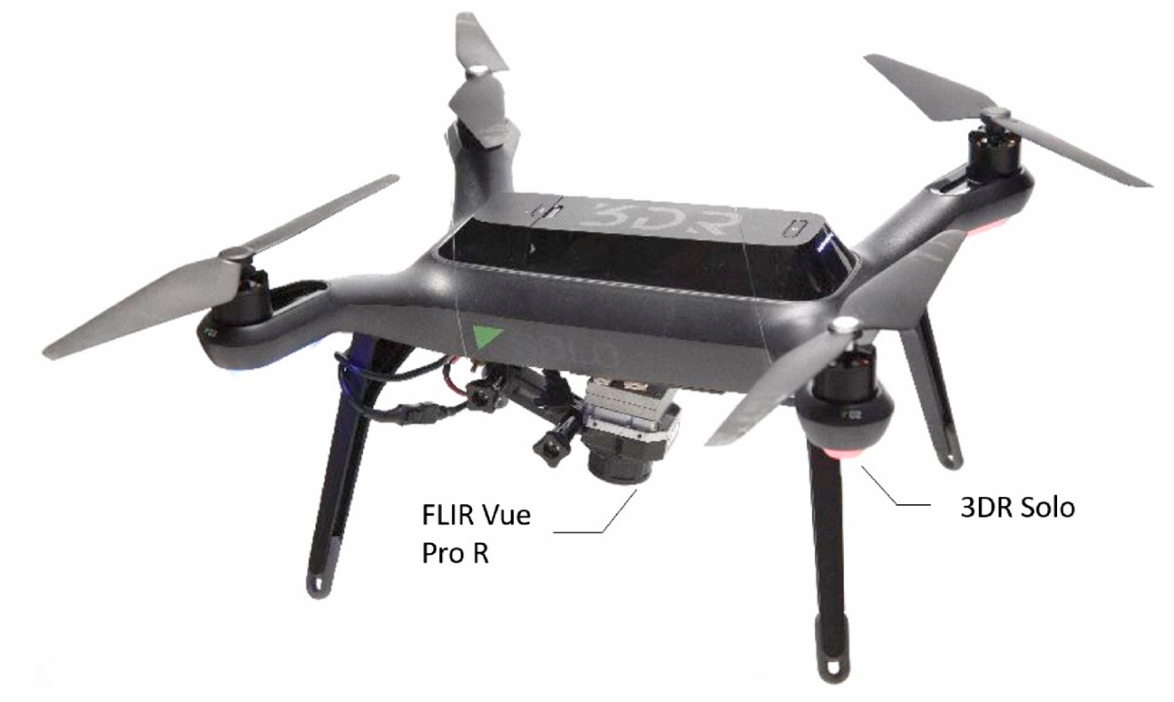
\includegraphics[width=\linewidth]{figs/Huirui/thermal_camera_drone.png}
        \caption{Thermal infrared camera mounted on UAV~\cite{nikulin2018detection}.}
        \label{fig:thermal_camera_drone}
    \end{subfigure}
    \hfill
    \begin{subfigure}[b]{0.48\linewidth}
        \centering
        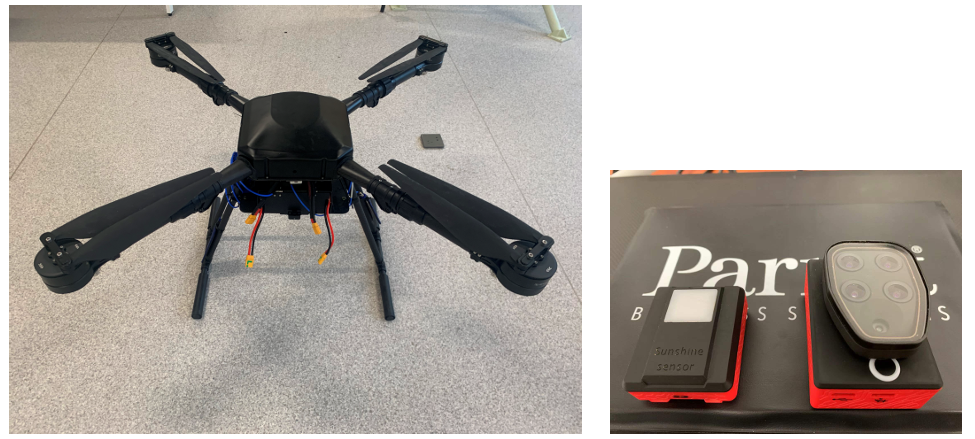
\includegraphics[width=\linewidth]{figs/Huirui/multispectral_drone.png}
        \caption{Multispectral camera mounted on UAV~\cite{qiu2023joint}.}
        \label{fig:optical_camera_drone}
    \end{subfigure}
    \caption{Examples of UAV-mounted spectral sensors used in landmine detection.}
    \label{fig:spectral_camera_drones}
\end{figure}


\paragraph{Mechanical and Vibro-Acoustic Methods}

This class includes detection technologies that exploit the mechanical or vibrational response of buried mines when stimulated by acoustic, seismic, or ultrasonic energy. These methods differ from electromagnetic and radar-based systems by relying on the physical compliance of buried objects rather than their electromagnetic properties~\cite{Gooneratne2004ARO,gichd2006guidebook}.

Acoustic and seismic techniques operate by transmitting low-frequency sound or seismic waves into the ground and measuring the reflected or re-radiated waves using contact or non-contact sensors. Mines are detected based on differences in their vibrational resonance, which contrasts with that of natural materials such as rocks, roots, or metal debris~\cite{gichd2006guidebook}. Similarly, ultrasound-based systems emit high-frequency acoustic waves (above 20 kHz) that reflect off material boundaries with different acoustic impedances. These reflections can be analyzed to image buried structures~\cite{paik2002image,cardonalandmine}.


\textbf{Drone-Based Applications:} No practical implementations have been reported to date. Research in this area is still at an early conceptual stage, with ground-based systems dominating current development.

\paragraph{Chemical and Biological Sensing Methods}

These techniques target the detection of explosive compounds or their vapors emitted by buried landmines. The methods include chemical vapor sensors, biosensors, and systems utilizing trained animals or genetically engineered microorganisms~\cite{Gooneratne2004ARO,alqudsi2021review}.

Biological methods involve using animals such as dogs, rats, or bees, or genetically modified bacteria that fluoresce in the presence of explosive molecules like TNT. Bacteria-based systems can be sprayed over a suspected minefield and monitored later for fluorescence~\cite{cardonalandmine}. Chemical sensors, by contrast, use materials such as polymer arrays or photoluminescent compounds to detect vapor signatures of explosives~\cite{alqudsi2021review}.


\textbf{Drone-Based Applications:} No fully developed or fielded systems have yet been reported in practice. Most developments in this area remain at the theoretical level.


\paragraph{Comparative Analysis and Method Selection}

The goal of this project is to develop a UAV-based landmine detection system capable of identifying both surface-laid and shallowly buried anti-personnel landmines. To ensure robustness and operational safety, the sensors should ideally be rigidly mounted onto the drone platform to minimize instability. Moreover, it is desirable to perform aerial scanning at altitudes greater than 1 meter to reduce the risk of ground collision and enhance area coverage efficiency. High scanning altitude improves flight safety and operational throughput but generally reduces the precision and resolution of subsurface sensing. Therefore, a careful trade-off is required between detection capability and system efficiency.

In this context, three main sensing modalities have been considered: magnetometers, GPR, and spectral imaging sensors (including optical, thermal, and hyperspectral/multispectral cameras). Additionally, other sensing methods such as biosensors and acoustic/vibro-mechanical sensors are excluded from detailed consideration due to their limited maturity for UAV integration. Existing research on biosensors and acoustic techniques for landmine detection remains largely theoretical, and no practical drone-based implementations have been reported to date.

\textbf{Magnetometer-Based Systems:} Magnetometers offer a lightweight and cost-effective option for detecting metallic landmines through magnetic anomaly measurements. However, they suffer from several operational constraints. To reliably detect small metallic objects, the UAV must fly at altitudes below 1 meter, which increases the risk of collisions and introduces challenges in maintaining flight stability~\cite{yoo2020drone,Yoo2024UnmannedAV}. Magnetic sensors are also susceptible to interference from the drone's motors and electronics, requiring physical separation of up to 1--2 meters from the UAV body~\cite{Yoo2024UnmannedAV,rs16162916}. This design increases system complexity and degrades stability, especially in dense environments. Additionally, these systems are ineffective against plastic or low-metal content landmines~\cite{garcia2020airborne,vsipovs2020lightweight}, and they lack imaging capabilities, limiting their utility for buried target identification~\cite{lee2023modeling}.

\textbf{Ground-Penetrating Radar (GPR):} GPR systems are highly effective for detecting both metallic and non-metallic buried landmines~\cite{vsipovs2020lightweight,colorado2017integrated}. They are relatively insensitive to surface clutter and can be used in all-weather, day/night operations~\cite{noviello2022overview}. However, their performance degrades significantly in highly conductive or moist soils~\cite{lee2023modeling}, and in the presence of rough or cluttered terrain~\cite{yoo2021application}. UAV-based GPR systems face challenges in signal attenuation due to altitude and scattering from the air-soil interface~\cite{garcia2019autonomous}. Although recent advancements have produced lightweight GPR units (e.g., 250 g with 5 W power consumption)~\cite{colorado2017integrated}, they still require low-altitude operation (0.5--2.5 m) to detect small or shallow mines accurately~\cite{vsipovs2020lightweight,colorado2017integrated,fernandez2021development}.

\textbf{Spectral Imaging Sensors:} Optical, thermal, hyperspectral, and multispectral cameras provide high-resolution imaging for detecting surface-laid mines or anomalies caused by disturbed soil and vegetation. They can also be flown at high altitudes, enabling efficient scanning of large areas. Optical (RGB) cameras are inexpensive and lightweight but are ineffective for detecting buried objects and suffer from high false negative rates in areas with dense vegetation~\cite{Baur2021HowTI,6842242,rs16122046}. Hyperspectral and multispectral systems offer enhanced material discrimination and are useful for identifying subtle spectral changes~\cite{10765909}. Although hyperspectral sensors theoretically cover a wide spectral range, including near and shortwave infrared, they are typically not optimized for the long wave infrared (LWIR) band required to detect subsurface thermal anomalies~\cite{ptsa-qj43-23}. More importantly, these systems are significantly more expensive than thermal infrared cameras, with reported costs being roughly twelve times higher, which limits their practical deployment on UAVs for widespread demining applications~\cite{rs15040967}. Among all spectral options, thermal infrared imaging has shown the most promise for detecting both surface and shallowly buried landmines due to differences in thermal inertia and conductivity between disturbed and undisturbed soil~\cite{ptsa-qj43-23,10.1117/12.2177182,Fardoulis2020PROOFHS}. UAV-mounted thermal cameras can be flown at altitudes of 5--10 meters and still achieve satisfactory detection accuracy for shallow targets under favorable environmental conditions~\cite{TENORIOTAMAYO2024105567,rs15040967}.

\textbf{Proposed Layered Detection Architecture:} Given the operational requirements and individual limitations of each sensor type, no single sensing modality provides a complete solution. Magnetometers are limited to low altitudes and metallic targets; GPR systems, while versatile, are sensitive to terrain and moisture and require low-altitude flights; and optical or hyperspectral sensors cannot detect buried targets reliably. Therefore, a layered sensing architecture is proposed.

In this framework, a thermal infrared camera operating at 5--10 meters altitude is used to perform an initial wide-area scan. Owing to its ability to detect both surface and shallowly buried landmines at high altitudes, the thermal camera effectively identifies thermally anomalous zones for further investigation. Subsequently, a UAV-mounted GPR unit is deployed at lower altitudes (1--5 meters) to conduct detailed subsurface scanning over the suspected regions. This radar system is selected for its ability to detect both metallic and non-metallic landmines with high resolution. By combining the efficiency and coverage of thermal imaging with the accuracy and material-agnostic detection of GPR, the proposed approach ensures both operational efficiency and robust landmine identification. The specific types and parameters of the thermal and GPR sensors used in this system, along with their corresponding flight configurations, will be discussed in the following sections.